% Generated by scripts/build_rq1_rq2_results.py — do not edit by hand.
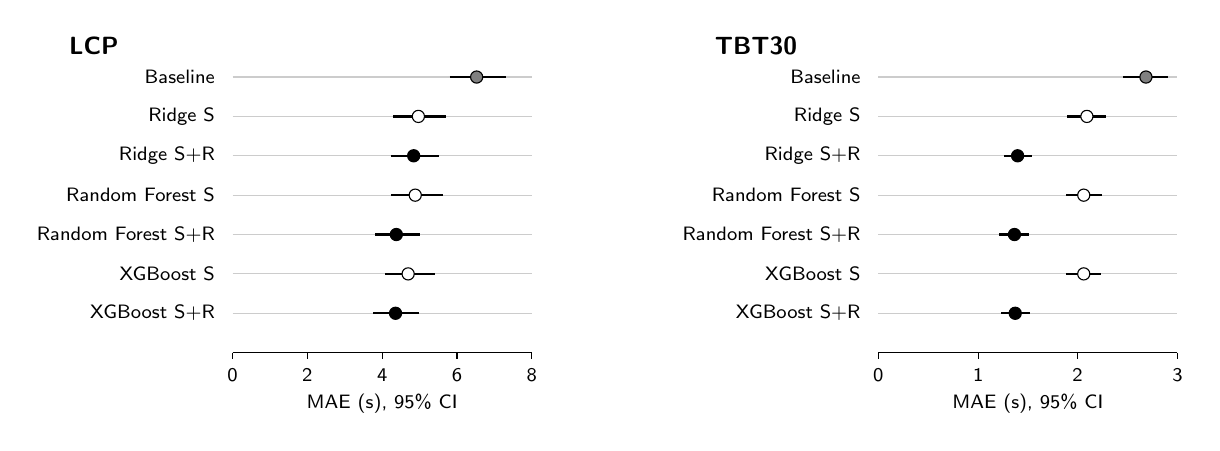
\begin{tikzpicture}[font=\sffamily\scriptsize]
\node[font=\sffamily\bfseries\small, anchor=west] at (0.0,3.9) {LCP};
\draw (2.20,0) -- (6.00,0);
\draw (2.20,0) -- (2.20,-0.08) node[below] {0};
\draw (3.15,0) -- (3.15,-0.08) node[below] {2};
\draw (4.10,0) -- (4.10,-0.08) node[below] {4};
\draw (5.05,0) -- (5.05,-0.08) node[below] {6};
\draw (6.00,0) -- (6.00,-0.08) node[below] {8};
\node at (4.10,-0.65) {MAE (s), 95\% CI};
\node[anchor=east] at (2.10,3.50) {Baseline};
\draw[gray!40] (2.20,3.50) -- (6.00,3.50);
\draw[thick] (4.96,3.50) -- (5.67,3.50);
\draw[fill=gray] (5.30,3.50) circle (2.2pt);
\node[anchor=east] at (2.10,3.00) {Ridge S};
\draw[gray!40] (2.20,3.00) -- (6.00,3.00);
\draw[thick] (4.24,3.00) -- (4.91,3.00);
\draw[fill=white] (4.56,3.00) circle (2.2pt);
\node[anchor=east] at (2.10,2.50) {Ridge S+R};
\draw[gray!40] (2.20,2.50) -- (6.00,2.50);
\draw[thick] (4.21,2.50) -- (4.82,2.50);
\draw[fill=black] (4.50,2.50) circle (2.2pt);
\node[anchor=east] at (2.10,2.00) {Random Forest S};
\draw[gray!40] (2.20,2.00) -- (6.00,2.00);
\draw[thick] (4.21,2.00) -- (4.87,2.00);
\draw[fill=white] (4.52,2.00) circle (2.2pt);
\node[anchor=east] at (2.10,1.50) {Random Forest S+R};
\draw[gray!40] (2.20,1.50) -- (6.00,1.50);
\draw[thick] (4.01,1.50) -- (4.58,1.50);
\draw[fill=black] (4.28,1.50) circle (2.2pt);
\node[anchor=east] at (2.10,1.00) {XGBoost S};
\draw[gray!40] (2.20,1.00) -- (6.00,1.00);
\draw[thick] (4.14,1.00) -- (4.77,1.00);
\draw[fill=white] (4.43,1.00) circle (2.2pt);
\node[anchor=east] at (2.10,0.50) {XGBoost S+R};
\draw[gray!40] (2.20,0.50) -- (6.00,0.50);
\draw[thick] (3.99,0.50) -- (4.57,0.50);
\draw[fill=black] (4.27,0.50) circle (2.2pt);
\node[font=\sffamily\bfseries\small, anchor=west] at (8.2,3.9) {TBT30};
\draw (10.40,0) -- (14.20,0);
\draw (10.40,0) -- (10.40,-0.08) node[below] {0};
\draw (11.67,0) -- (11.67,-0.08) node[below] {1};
\draw (12.93,0) -- (12.93,-0.08) node[below] {2};
\draw (14.20,0) -- (14.20,-0.08) node[below] {3};
\node at (12.30,-0.65) {MAE (s), 95\% CI};
\node[anchor=east] at (10.30,3.50) {Baseline};
\draw[gray!40] (10.40,3.50) -- (14.20,3.50);
\draw[thick] (13.51,3.50) -- (14.08,3.50);
\draw[fill=gray] (13.80,3.50) circle (2.2pt);
\node[anchor=east] at (10.30,3.00) {Ridge S};
\draw[gray!40] (10.40,3.00) -- (14.20,3.00);
\draw[thick] (12.80,3.00) -- (13.29,3.00);
\draw[fill=white] (13.05,3.00) circle (2.2pt);
\node[anchor=east] at (10.30,2.50) {Ridge S+R};
\draw[gray!40] (10.40,2.50) -- (14.20,2.50);
\draw[thick] (12.00,2.50) -- (12.35,2.50);
\draw[fill=black] (12.17,2.50) circle (2.2pt);
\node[anchor=east] at (10.30,2.00) {Random Forest S};
\draw[gray!40] (10.40,2.00) -- (14.20,2.00);
\draw[thick] (12.79,2.00) -- (13.24,2.00);
\draw[fill=white] (13.01,2.00) circle (2.2pt);
\node[anchor=east] at (10.30,1.50) {Random Forest S+R};
\draw[gray!40] (10.40,1.50) -- (14.20,1.50);
\draw[thick] (11.94,1.50) -- (12.32,1.50);
\draw[fill=black] (12.13,1.50) circle (2.2pt);
\node[anchor=east] at (10.30,1.00) {XGBoost S};
\draw[gray!40] (10.40,1.00) -- (14.20,1.00);
\draw[thick] (12.79,1.00) -- (13.23,1.00);
\draw[fill=white] (13.01,1.00) circle (2.2pt);
\node[anchor=east] at (10.30,0.50) {XGBoost S+R};
\draw[gray!40] (10.40,0.50) -- (14.20,0.50);
\draw[thick] (11.96,0.50) -- (12.33,0.50);
\draw[fill=black] (12.14,0.50) circle (2.2pt);
\end{tikzpicture}